\documentclass{ltjsarticle}
\usepackage{amsmath}
\usepackage{graphicx}
\usepackage{geometry}
\usepackage{float}
\usepackage{hyperref}
\usepackage{url}
\geometry{left=25mm,right=25mm,top=25mm,bottom=25mm}

\begin{document}
\title{論理回路}
\author{平野 健汰}
\date{\today}

\maketitle

\section{目的}
ディジタルシステムを構成する論理回路について,組み合わせ回路,順序回路の動作と設計法・実装法の実習,論理素子の動作の理解.

\section{理論}
\subsection{ディジタル信号処理と論理素子}
ディジタル信号処理を行うデバイスは多岐にわたるが,その主要部分は論理回路である.
つまり,二値論理とそれを実行する論理素子からなる.
論理素子の実態は電磁リレーや真空管,バイポーラトランジスタなどの連続した入出力特性を持つスイッチング回路である.
そして,素子ごとに固有の電気的,時間的特性を持つ.
このため,高速な動作を行うディジタル信号処理回路を設計・作製するためにはこれらの特性を考慮する必要がある.

\subsection{論理素子(CMOS)の特性}
\subsubsection{動作電圧範囲(最大定格,推奨動作条件)}
ディジタルICにはIC毎に決まった動作保証に関する電気的条件がある.
これは,電源電圧,動作周波数,動作温度範囲などがある.
その条件を満足するように使う必要がある.

\noindent 絶対最大定格:端子に印加できる最大の電圧,あるいは流すことができる最大の電流.
これはICの破壊を防ぐために必ず守らなければならない.

\noindent 推奨動作条件:ICが正常に動作するための電気的条件.
これは,ICの性能を最大限に引き出すために守るべき条件である.

\subsubsection{入出力電圧特性(${V_{OH}, V_{OL}, V_{IH}, V_{IL}}$)}
ディジタルICはアナログ値を持つ入出力電圧が,高レベルか低レベルかを判定して信号処理を行う.
\begin{itemize}
  \item ${V_{OH}}$:出力ハイレベル電圧
  \item ${V_{OL}}$:出力ローレベル電圧
  \item ${V_{IH}}$:入力ハイレベル電圧
  \item ${V_{IL}}$:入力ローレベル電圧
\end{itemize}

\subsubsection{伝搬遅延時間}
伝搬遅延時間とは入力状態に変化を加えた場合,出力状態が変化するのにかかる時間を表す特性である.
\begin{itemize}
  \item ${t_{PLH}}$:ローレベルからハイレベルへの伝搬遅延時間
  \item ${t_{PHL}}$:ハイレベルからローレベルへの伝搬遅延時間
  \item ${t_{pd}}$:${t_{PLH}}$と${t_{PHL}}$の平均
\end{itemize}

\subsubsection{ファンアウト}
ファンアウトとは,ある素子が特性を満たす範囲で駆動できる同一の素子の数を表す.
ファンアウトが大きいほど,多くの素子を駆動できるが,伝搬遅延時間が大きくなる.


\section{使用器具}
\begin{itemize}
  \item LED: 4個
  \item ジャンプワイヤ: 一式
  \item 抵抗器(330 $\Omega$): 4個,(1 k$\Omega$): 4個
  \item コンデンサ(470 nF): 3個,(4.7 $\mu$F): 3個
  \item タクトスイッチ: 1個
  \item Dフリップフロップ IC (TC74AC74P, Toshiba): 1個
  \item 2入力論理和 IC (TC74HC08AP, Toshiba): 1個
  \item インバータ IC (TC74HC14AP, Toshiba): 1個
\end{itemize}

\section{実験}
\subsection{実験方法}
\subsubsection{リングオシレータ}
\begin{itemize}
  \item ブレッドボード上にインバータ回路をロジックIC(インバータ)を用いて実装した.
  \item 2種類のコンデンサ(470 nF, 4.7 $\mu$F)を用いてファンクションジェネレータより方形波(f = 100 Hz, Vpp = 5 V, offset = 2.5 V)を入力した.
  \item 出力波形をオシロスコープで観測した.
\end{itemize}

\begin{itemize}
  \item ブレッドボード上に三段の縦続接続インバータによるリングオシレータ回路を実装した.
  \item V1, V2 を観測して1素子の伝搬遅延時間,発振周波数を求めた.
  \item 各段のコンデンサを変更して同様に測定した.
\end{itemize}

\subsubsection{Dフリップフロップを用いた2ビット4進非同期カウンタ回路}
\begin{itemize}
  \item ブレッドボード上に2ビットカウンタ回路をロジックIC(エッジトリガ型Dフリップフロップ)を用いて実装した.
  \item ファンクションジェネレータ(f = 1 kHz, Vpp = 5 V, offset = 2.5 V の方形波)をクロック信号CLKとして用いて駆動させた.
  \item Q1, Q2 およびクロック CLK を観測して記録した.
\end{itemize}

\subsubsection{2ビットデコーダ回路によるLEDルーレット}
\begin{itemize}
  \item ブレッドボード上に2ビットデコーダ回路と LED 回路をロジックIC(2入力論理和)を用いて実装した.
  \item 2bit4 進カウンタ回路と接続し,FG(f = 10 Hz, Vpp = 5 V, offset = 2.5 V の方形波)をクロック信号CLKとして用いて駆動させた.
  \item LED の点灯状態を観測して動画で記録した.
  \item LED の光る順番を記録した.
\end{itemize}

\begin{itemize}
  \item リングオシレータと2ビット4 進非同期カウンタ回路を接続した.
  \item 間にはタクトスイッチを挟んだ.
  \item タクトスイッチが推されている間,LED がルーレットのように点滅し,スイッチをオフにすると4つのLEDのうち1つのLEDのみが点灯することを確認し,記録した.
\end{itemize}

\subsection{結果}
\subsubsection{実験課題1}
\begin{table}[H]
\centering
\begin{tabular}{|c|c|}
\hline
コンデンサ[${\mu F}$] & 遅延時間[${ms}$] \\ \hline
4.7 & 7.62  \\ \hline
0.47 & 5.56 \\ \hline
\end{tabular}
\caption{ファンクションジェネレータを利用したリングオシレータのコンデンサと遅延時間の関係}
\label{tab:results_1}
\end{table}

\begin{figure}[H]
\centering
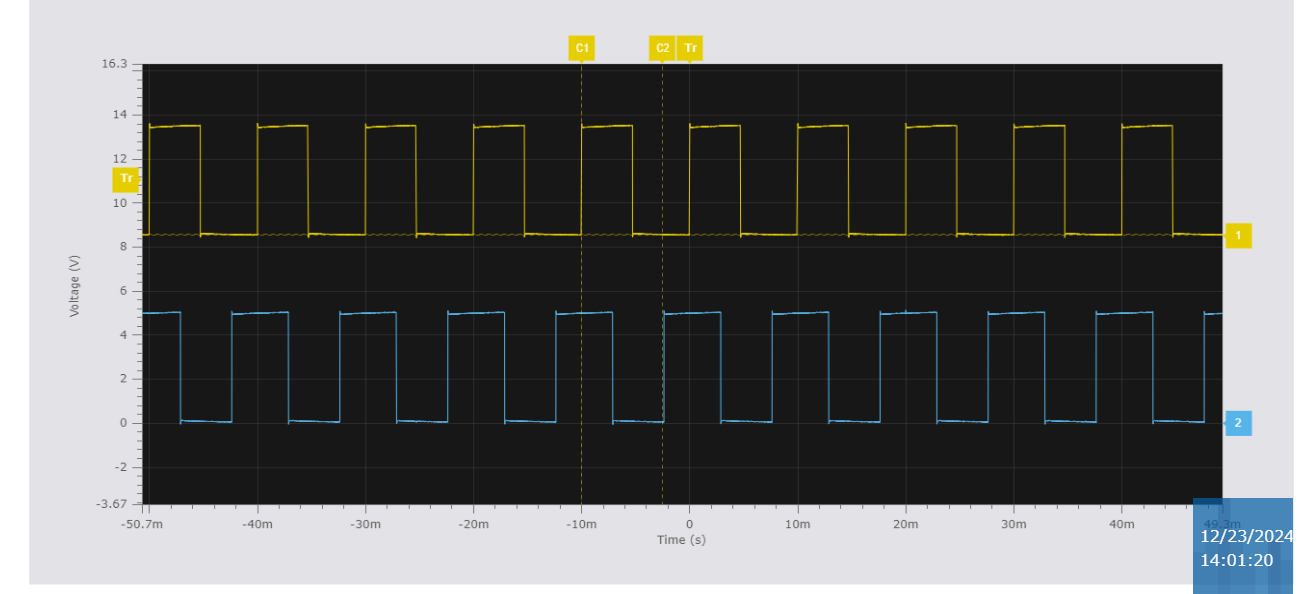
\includegraphics[width=0.8\textwidth]{figs/1-4700nF.png}
\caption{4.7 $\mu$F のコンデンサを用いたリングオシレータの波形}
\label{fig:1_4.7_experiment_results}
\end{figure}

\begin{figure}[H]
  \centering
  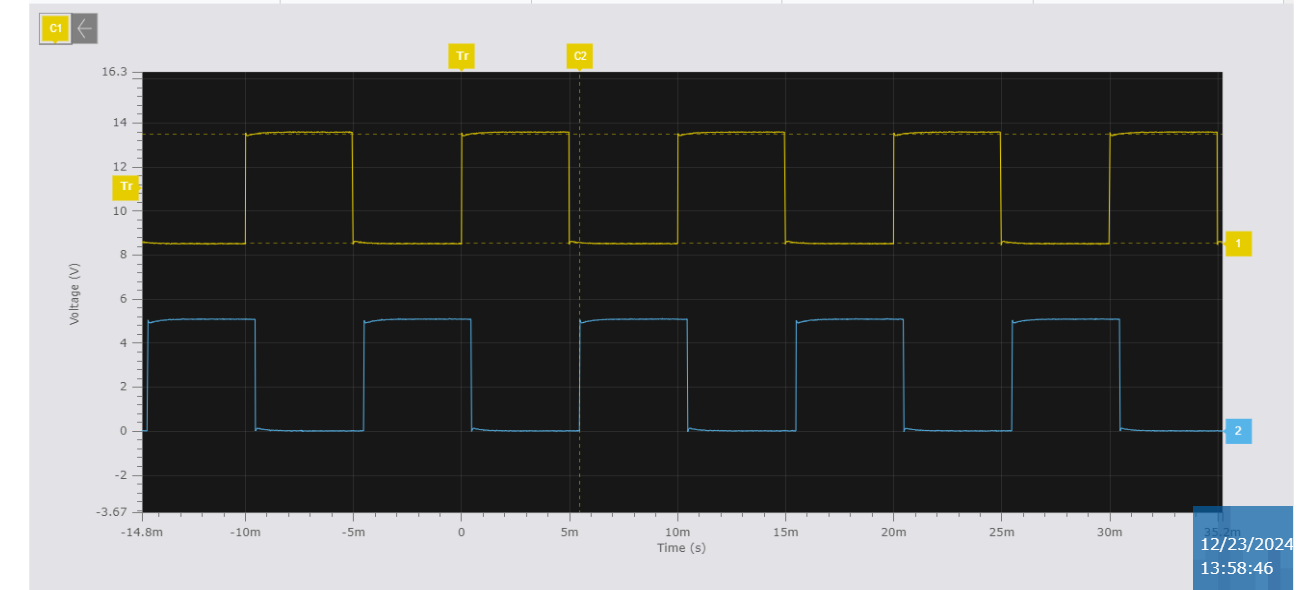
\includegraphics[width=0.8\textwidth]{figs/1-470mF.png}
  \caption{470 nF のコンデンサを用いたリングオシレータの波形}
  \label{fig:1_470_experiment_results}
  \end{figure}

\subsubsection{実験課題2}
\begin{table}[H]
  \centering
  \begin{tabular}{|c|c|}
  \hline
  コンデンサ[${\mu F}$] & 遅延時間[${ms}$] \\ \hline
  4.7 & 16.7  \\ \hline
  0.47 & 1.77 \\ \hline
  \end{tabular}
  \caption{リングオシレータのコンデンサと遅延時間の関係}
  \label{tab:results_2}
\end{table}

\begin{figure}[H]
  \centering
  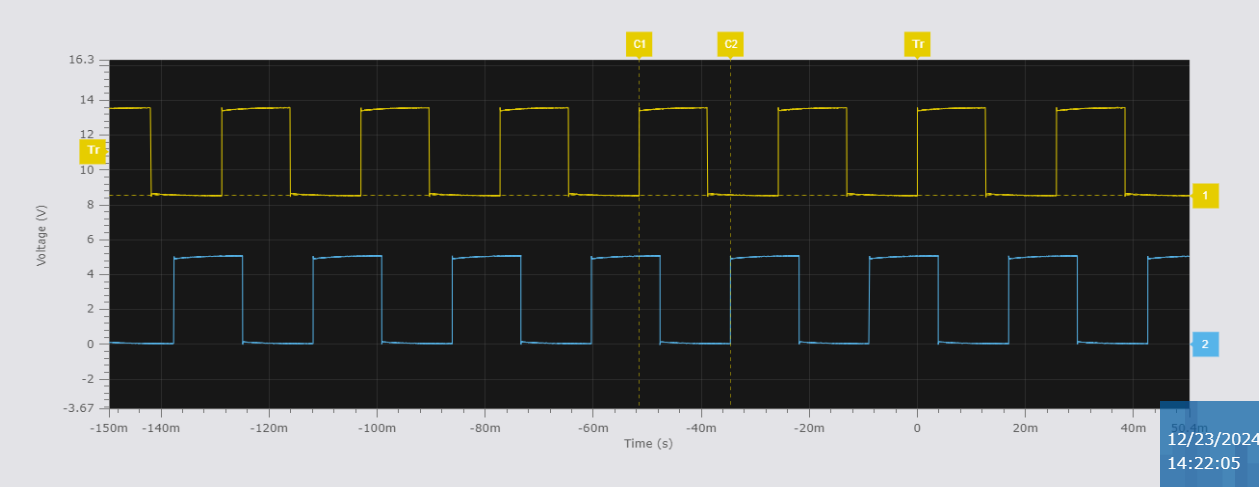
\includegraphics[width=0.8\textwidth]{figs/2-4700nF.png}
  \caption{4.7 $\mu$F のコンデンサを用いたリングオシレータの波形}
  \label{fig:2_4.7_experiment_results}
\end{figure}

\begin{figure}[H]
  \centering
  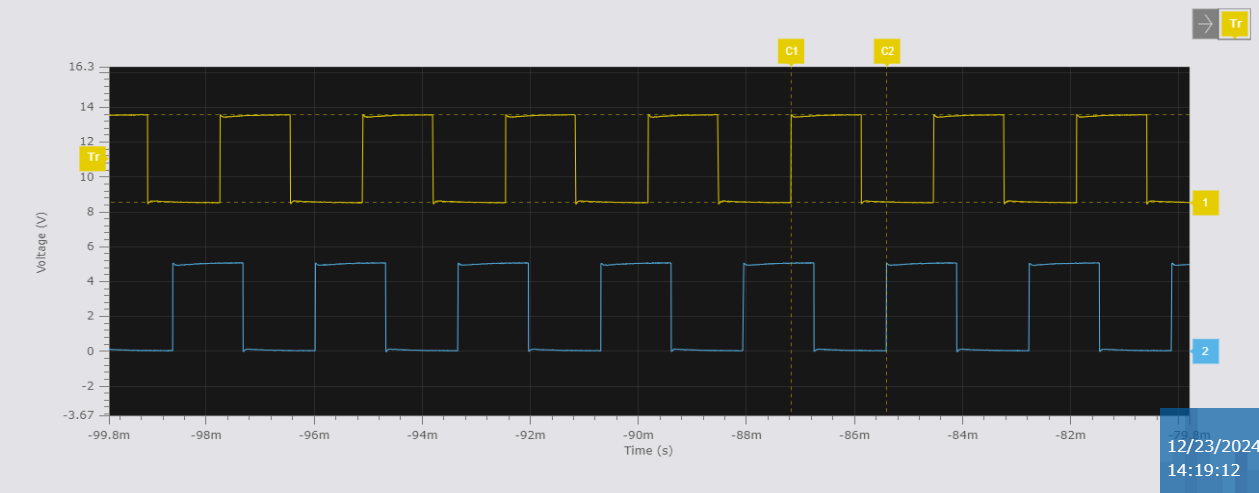
\includegraphics[width=0.8\textwidth]{figs/2-470nF.png}
  \caption{470 nF のコンデンサを用いたリングオシレータの波形}
  \label{fig:2_470_experiment_results}
\end{figure}

\subsubsection{実験課題3}
\begin{figure}[H]
  \centering
  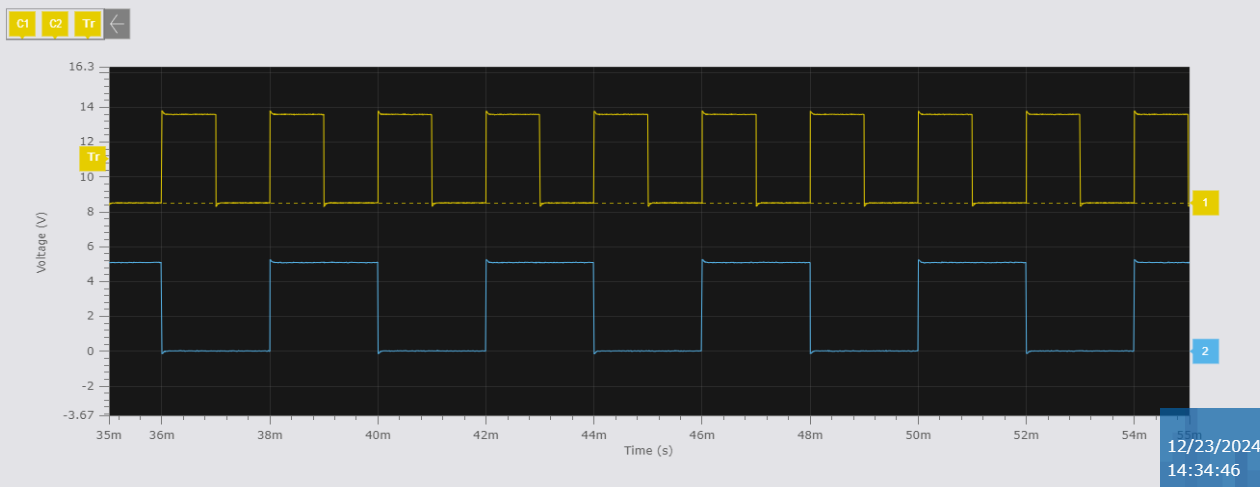
\includegraphics[width=0.8\textwidth]{figs/3-flipflop.png}
  \caption{2ビット4進非同期カウンタ回路の波形}
  \label{fig:3_experiment_results}
\end{figure}

\subsubsection{実験課題4}
LEDの光る順番は LED4 → LED3 → LED2 → LED1 → LED4 → ・・・ となった.

\section{考察}
\subsection{基本課題(1) インバータIC回路}
表\ref{tab:results_1}より,コンデンサの容量が大きいほど遅延時間が大きくなることがわかる.
これは,コンデンサの容量が大きいほど,充放電にかかる時間が大きくなるためである.

\subsection{基本課題(2) リングオシレータ}
\begin{table}[H]
\centering
\begin{tabular}{|c|c|c|c|}
\hline
コンデンサ[${\mu F}$] & 伝達遅延時間[${ms}$] & 全体の伝達遅延時間[${ms}$] & 発振周波数[${Hz}$] \\ \hline
4.7 & 16.7 & 50.1 & 38.9  \\ \hline
0.47 & 1.77 & 5.31 & 379 \\ \hline
\end{tabular}
\caption{リングオシレータのコンデンサと遅延時間,発振周波数の関係}
\label{tab:discussion_results}
\end{table}

表\ref{tab:discussion_results}より,コンデンサの容量が大きいほど遅延時間が大きくなり,発振周波数が小さくなることがわかる.
これは,コンデンサの容量が大きいほど,充放電にかかる時間が大きくなるためである.
つまり,発振周波数をより早くするためには,コンデンサの容量を小さくする必要がある.

\subsection{基本課題(3) 2ビット4進非同期カウンタ回路}
図\ref{fig:3_experiment_results}より,2ビット4進非同期カウンタ回路の波形が正常に動作していることがわかる.
この回路が2ビット4進カウンタになることを説明する.
この回路は,2つのDフリップフロップを用いて,2ビットのカウンタを実装している.
このカウンタは,クロック信号が入力されるたびに,カウンタが1つ進む.
図\ref{fig:3_experiment_results}より,Q1, Q2の値が変化していて,4つの状態を持つことがわかる.
以上より,この回路は2ビット4進カウンタになることがわかる.
\begin{figure}[H]
  \centering
  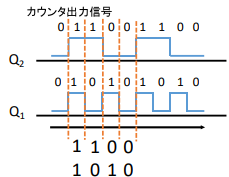
\includegraphics[width=0.8\textwidth]{figs/ringosilator.png}
  \caption{2ビット4進非同期カウンタ回路の波形}
  \label{fig:3_experiment_results}
\end{figure}

\subsection{基本課題(4) LED用デコーダ回路及び電子ルーレット}
2ビット4進非同期カウンタ回路とデコーダ回路で電子ルーレットになる仕組みについて述べる.
先述のとおり,2ビット4進非同期カウンタ回路は,2ビットのカウンタを実装している.
つまり,4つの状態を持ち,クロック信号が入力されるたびに,1つの状態に進む.
このカウンタの出力をデコーダ回路に入力すると,4つの状態を表す信号が1つだけハイレベルになる.
この信号をLEDに入力することで,LEDが点灯する.
このため,この回路は,4つのLEDのうち1つのLEDのみが点灯する電子ルーレットとなる.

\vspace{\baselineskip}
次にLEDの光る順番について考察する.
この回路は,2ビット4進非同期カウンタ回路を用いているため,4つの状態を持つ.
\begin{itemize}
  \item LED1は,$\overline{Q_2}$と$\overline{Q_1}$の論理和である.
  \item LED2は,$\overline{Q_2}$と${Q_1}$の論理和である.
  \item LED3は,${Q_2}$と$\overline{Q_1}$の論理和である.
  \item LED4は,${Q_2}$と${Q_1}$の論理和である.
\end{itemize}
${Q_2}$の値が1のとき,${Q_1}$の値は0から1に変化する.
その後,${Q_2}$の値が0になり,${Q_1}$の値は1から0に変化する.
このため,LEDの光る順番は,LED4 → LED3 → LED2 → LED1 → LED4 → ・・・ となる.

\vspace{\baselineskip}
次にLEDがルーレットのように光る間隔とリングオシレーターが作るクロック信号及びFGの波形の周波数との関係について考察する.
リングオシレーターは,クロック信号を入力すると,その周波数に合わせて発振する.
このため,リングオシレーターの周波数が高いほど,LEDがルーレットのように光る間隔が速くなる.
また,リングオシレーターの周波数が低いほど,LEDがルーレットのように光る間隔が遅くなる.

\subsection{基本課題(5)}
デジタルICとして,携帯電話(スマートフォン)に用いられている.ICチップの大幅な削減や,機器の小型化,省電力化に貢献している.
また,デジタルICは,高速な動作が可能であるため,高速なデータ処理が可能である.
これにより,高速なデータ通信や,高速な画像処理が可能になっている.
% デジタルICについて参照を書く

\begin{thebibliography}{9}
\bibitem{reference1} \url{https://example.com/reference1}
\end{thebibliography}

\end{document}